\documentclass[border=4mm]{article}
\usepackage{tikz}
\usetikzlibrary{arrows.meta,positioning}
\title{Ford Fulkerson Algorithm for Max Flow}
\begin{document}
    \maketitle
    \tableofcontents
    \section{Maximum Flow}
    A Maximum-Flow is the flow of maximum possible value from source to sink.

    \section{Flow Network}
    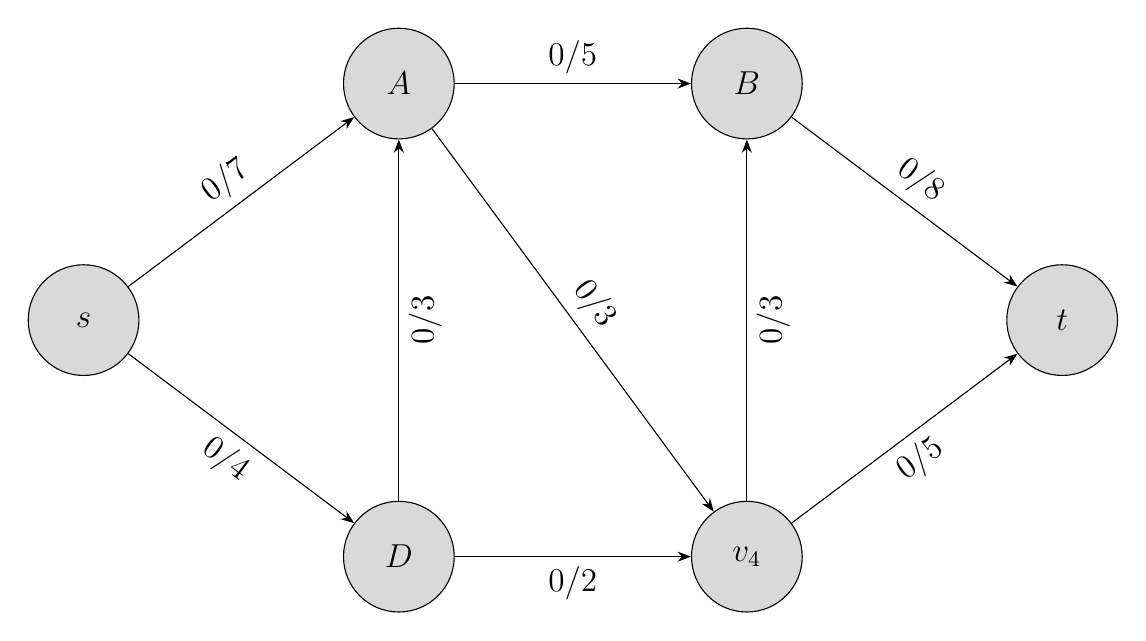
\begin{tikzpicture}[
        mycircle/.style={
        circle,
        draw=black,
        fill=gray,
        fill opacity = 0.3,
        text opacity=1,
        inner sep=2pt,
        minimum size=40pt,
        font=\large},
    myarrow/.style={-Stealth},
    node distance=2cm and 3cm
    ]
    \node[mycircle] (c1) {$s$};
    \node[mycircle,below right=of c1] (c2) {$D$};
    \node[mycircle,right=of c2] (c3) {$v_4$};
    \node[mycircle,above right=of c1] (c4) {$A$};
    \node[mycircle,right=of c4] (c5) {$B$};
    \node[mycircle,below right=of c5] (c6) {$t$};

    \foreach \i/\j/\txt/\p in {% start node/end node/text/position
        c1/c2/{0/4}/below,
        c1/c4/{0/7}/above,
        c2/c3/{0/2}/below,
        c3/c6/{0/5}/below,
        c4/c5/{0/5}/above,
        c5/c6/{0/8}/above,
        c3/c5/{0/3}/below,
        c2/c4/{0/3}/below,
        c4/c3/{0/3}/above}
        \draw [myarrow] (\i) -- node[sloped,font=\large,\p] {\txt} (\j);


    % draw this outside loop to get proper orientation of 10
    \end{tikzpicture}

    \section{Maximum-flow in the network}
    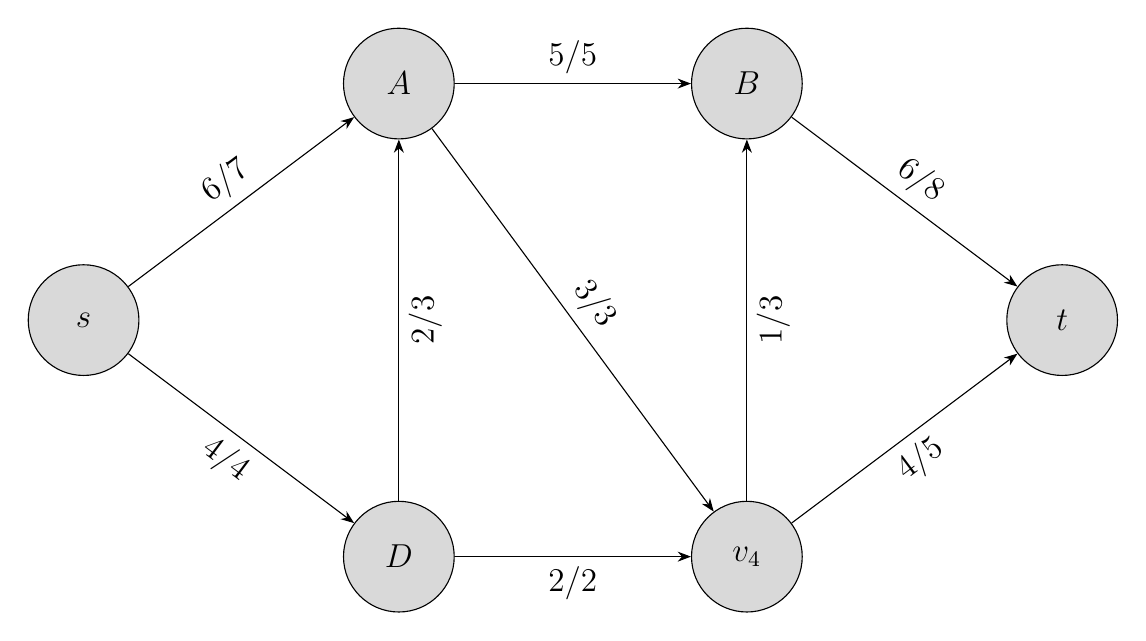
\begin{tikzpicture}[
        mycircle/.style={
        circle,
        draw=black,
        fill=gray,
        fill opacity = 0.3,
        text opacity=1,
        inner sep=2pt,
        minimum size=40pt,
        font=\large},
    myarrow/.style={-Stealth},
    node distance=2cm and 3cm
    ]
    \node[mycircle] (c1) {$s$};
    \node[mycircle,below right=of c1] (c2) {$D$};
    \node[mycircle,right=of c2] (c3) {$v_4$};
    \node[mycircle,above right=of c1] (c4) {$A$};
    \node[mycircle,right=of c4] (c5) {$B$};
    \node[mycircle,below right=of c5] (c6) {$t$};

    \foreach \i/\j/\txt/\p in {% start node/end node/text/position
        c1/c2/{4/4}/below,
        c1/c4/{6/7}/above,
        c2/c3/{2/2}/below,
        c3/c6/{4/5}/below,
        c4/c5/{5/5}/above,
        c5/c6/{6/8}/above,
        c3/c5/{1/3}/below,
        c2/c4/{2/3}/below,
        c4/c3/{3/3}/above}
        \draw [myarrow] (\i) -- node[sloped,font=\large,\p] {\txt} (\j);


    % draw this outside loop to get proper orientation of 10
    \end{tikzpicture}

    \section{Reverse Edge \& Residual Capacity}

    \subsection{Residual Capacity}
        Residual Capacity of an edge is defined as the capacity minus flow.

    \subsection{Reverse Edge Residual Capacity}
        Residual Capacity of reverse edge is defined as the capacity of reverse edge minus flow in reverse edge.

        If flow of edge (u, v) = x 

        Then flow of edge (v, u) = -x

        Capacity of reverse edge = 0
        \begin{figure}
        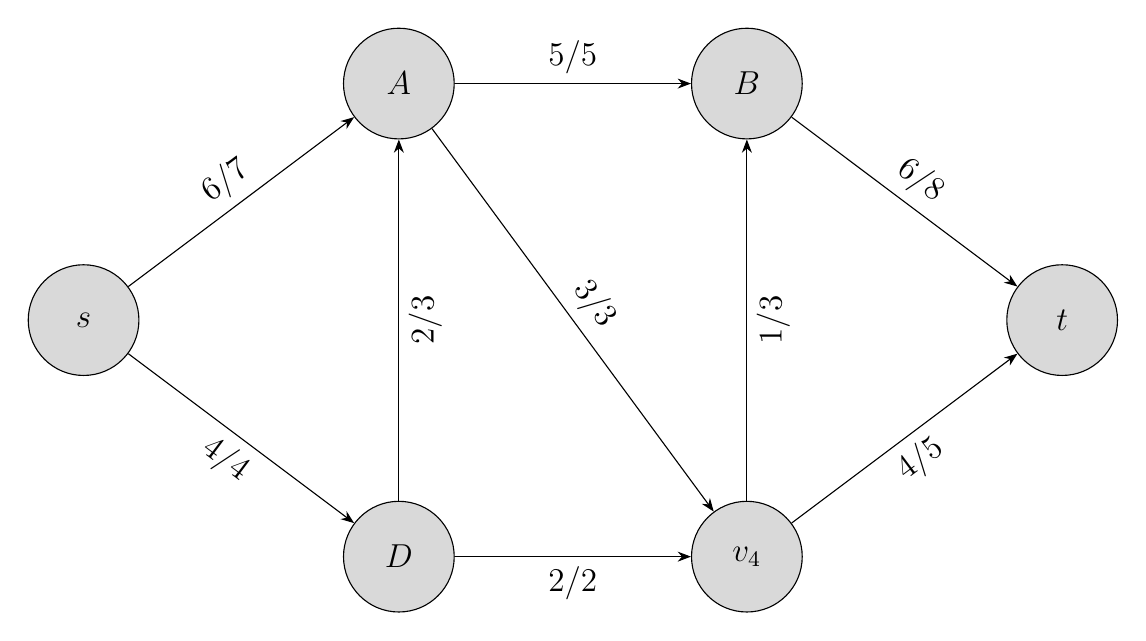
\begin{tikzpicture}[
            mycircle/.style={
            circle,
            draw=black,
            fill=gray,
            fill opacity = 0.3,
            text opacity=1,
            inner sep=2pt,
            minimum size=40pt,
            font=\large},
        myarrow/.style={-Stealth},
        node distance=2cm and 3cm
        ]
        \node[mycircle] (c1) {$s$};
        \node[mycircle,below right=of c1] (c2) {$D$};
        \node[mycircle,right=of c2] (c3) {$v_4$};
        \node[mycircle,above right=of c1] (c4) {$A$};
        \node[mycircle,right=of c4] (c5) {$B$};
        \node[mycircle,below right=of c5] (c6) {$t$};
    
        \foreach \i/\j/\txt/\p in {% start node/end node/text/position
            c1/c2/{4/4}/below,
            c1/c4/{6/7}/above,
            c2/c3/{2/2}/below,
            c3/c6/{4/5}/below,
            c4/c5/{5/5}/above,
            c5/c6/{6/8}/above,
            c3/c5/{1/3}/below,
            c2/c4/{2/3}/below,
            c4/c3/{3/3}/above}
            \draw [myarrow] (\i) -- node[sloped,font=\large,\p] {\txt} (\j);
    
    
        % draw this outside loop to get proper orientation of 10
        \end{tikzpicture}
        \caption{Original Graph}
    \end{figure}

    \begin{figure}
        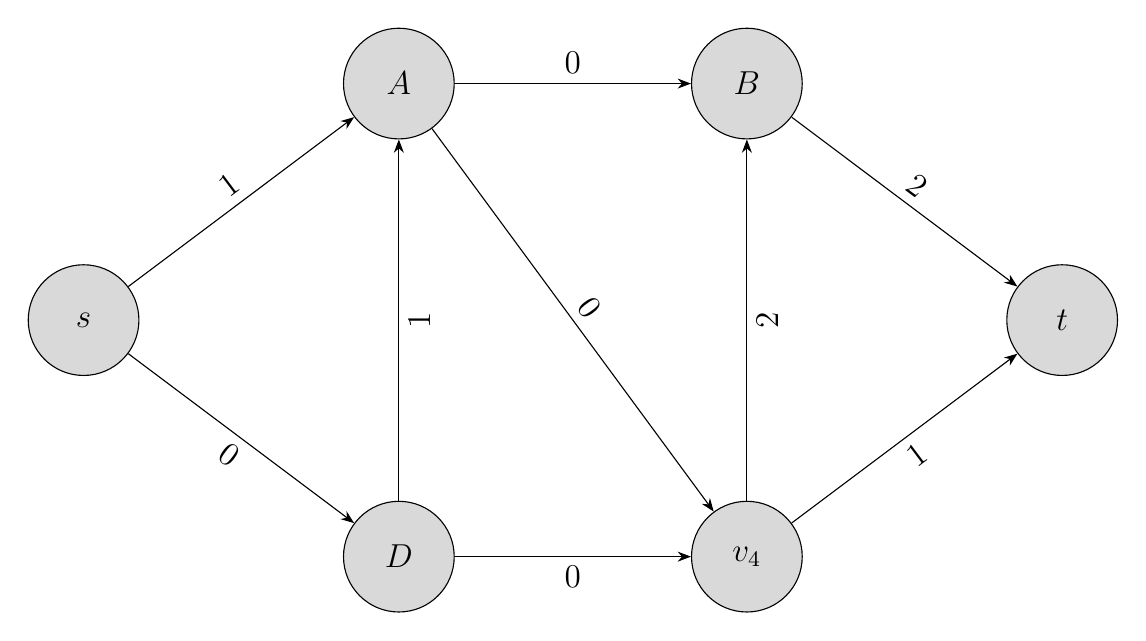
\begin{tikzpicture}[
            mycircle/.style={
            circle,
            draw=black,
            fill=gray,
            fill opacity = 0.3,
            text opacity=1,
            inner sep=2pt,
            minimum size=40pt,
            font=\large},
        myarrow/.style={-Stealth},
        node distance=2cm and 3cm
        ]
        \node[mycircle] (c1) {$s$};
        \node[mycircle,below right=of c1] (c2) {$D$};
        \node[mycircle,right=of c2] (c3) {$v_4$};
        \node[mycircle,above right=of c1] (c4) {$A$};
        \node[mycircle,right=of c4] (c5) {$B$};
        \node[mycircle,below right=of c5] (c6) {$t$};
    
        \foreach \i/\j/\txt/\p in {% start node/end node/text/position
            c1/c2/{0}/below,
            c1/c4/{1}/above,
            c2/c3/{0}/below,
            c3/c6/{1}/below,
            c4/c5/{0}/above,
            c5/c6/{2}/above,
            c3/c5/{2}/below,
            c2/c4/{1}/below,
            c4/c3/{0}/above}
            \draw [myarrow] (\i) -- node[sloped,font=\large,\p] {\txt} (\j);
    
    
        % draw this outside loop to get proper orientation of 10
        \end{tikzpicture}
        \caption{Residual Capacity}
    \end{figure}

    \begin{figure}
        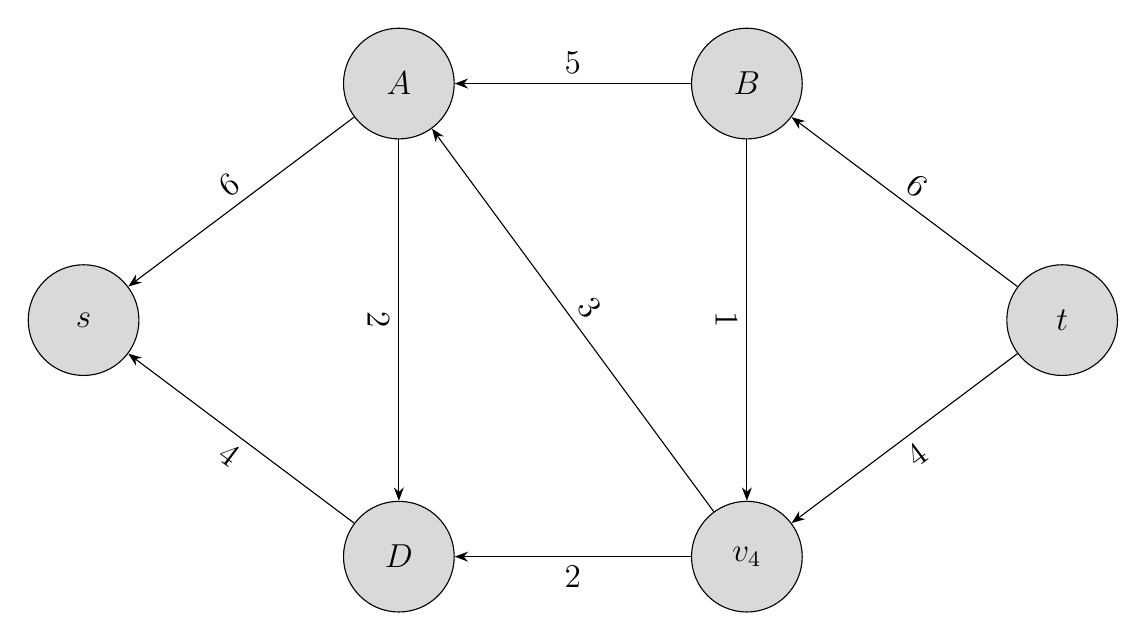
\begin{tikzpicture}[
            mycircle/.style={
            circle,
            draw=black,
            fill=gray,
            fill opacity = 0.3,
            text opacity=1,
            inner sep=2pt,
            minimum size=40pt,
            font=\large},
        myarrow/.style={-Stealth},
        node distance=2cm and 3cm
        ]
        \node[mycircle] (c1) {$s$};
        \node[mycircle,below right=of c1] (c2) {$D$};
        \node[mycircle,right=of c2] (c3) {$v_4$};
        \node[mycircle,above right=of c1] (c4) {$A$};
        \node[mycircle,right=of c4] (c5) {$B$};
        \node[mycircle,below right=of c5] (c6) {$t$};
    
        \foreach \i/\j/\txt/\p in {% start node/end node/text/position
            c2/c1/{4}/below,
            c4/c1/{6}/above,
            c3/c2/{2}/below,
            c6/c3/{4}/below,
            c5/c4/{5}/above,
            c6/c5/{6}/above,
            c5/c3/{1}/below,
            c4/c2/{2}/below,
            c3/c4/{3}/above}
            \draw [myarrow] (\i) -- node[sloped,font=\large,\p] {\txt} (\j);
    
    
        % draw this outside loop to get proper orientation of 10
        \end{tikzpicture}
        \caption{Reverse Edge Residual Capacity}
    \end{figure}
\end{document}